\chapter{Theory}

The theory chapter provides an overview of the preliminary theoretical groundwork, relevant for understanding the methodology employed. The first section of the mathematical foundation covers the underlying model statements and assumptions in linear models, extending onto GLMMs. Subsequently, we present the statistical models used in quantitative genetics. Lastly, we introduce the statistical framework used for model fitting, namely Bayesian statistics and INLA. 

\section{Mathematical foundation} 

\subsection{Linear models}
\label{sec:theory:linear model}
A linear model, hereafter denoted a Gaussian model, assumes that the continuous response variable $y$ is a linear combination of a given number of covariates, an error term and an intercept. Linear regression can be formulated as
\begin{equation}
y = \beta_0 + \sum_{i=1}^p \beta_i x_i + \varepsilon \,    
\label{eq:lin.reg scalar expression}
\end{equation}
where $y$ is the response variable, $x_i$ are observations for covariate $i$ out of the $p$ number of covariates, $\beta_i$ is the estimator for each covariate and $\varepsilon \sim \mathcal{N}(0,\sigma^2)$ is the error term. That is, $\varepsilon$ follows a standard normal distribution with mean $0$ and variance $\sigma^2$. Equivalently, linear regression in matrix notation generalizes to $n$ different responses using the design matrix $\bm X$, so that the expression becomes

\begin{align}
\label{eq:linear regression matrix}
\bm y &= \bm X \bm \beta + \bm \varepsilon \ , \; 
\bm y = [y_1, \dots, y_n]^\top \ , \; 
\bm \beta = [\beta_1, \dots, \beta_n]^\top \;
\bm \varepsilon = [\varepsilon_1, \dots, \varepsilon_n]^\top, \\
\bm X &= \begin{bmatrix}
1       & x_{11} & \cdots & x_{1p} \\
1       & x_{21} & \cdots & x_{2p} \\
\vdots  & \vdots & \ddots & \vdots \\
1       & x_{n1} & \cdots & x_{np} \nonumber
\end{bmatrix} \ .
\end{align}

Linear regression relies on four major assumptions. The first assumption, exogeneity, assumes that there is no error in the data from the design matrix, i.e. $\E{\bm \varepsilon | \bm X} = 0$. %$\operatorname{Corr}(\bm X, \bm \varepsilon) = 0$.
The second assumption is that the relationship between the response and the covariates is linear, indicated by equations \eqref{eq:lin.reg scalar expression} and \eqref{eq:linear regression matrix}. The third assumption is that the estimated errors $\bm e = \widehat{\bm y}-\bm y$, also called residuals, are independent and identically distributed (iid) as a normal distribution with mean zero and constant variance. Finally, we assume that we do not have perfect multicollinearity in the predictors, which means that the covariates are linearly dependent and $\operatorname{rank}(\bm X)$ is not full. Violating these assumptions can compromise the performance of the model and lead to biased estimators.

There are several advantages to using linear regression for inference. Firstly, the maximum likelihood estimator has the closed form
\begin{equation}
    \label{eq:theory:closed form linreg}
    \hat{\bm\beta} = (\bm X^\top \bm X)^{-1} \bm X^\top \bm y \ .
\end{equation}
As such, both implementation and interpretability of the model fit are relatively easy. There are several methods for evaluating model fit, and easy-to-use libraries in most modern programming languages already exist. Furthermore, due to the linear relationship between the covariates and the response variable, we can see that an increase of one unit in $\bm x_{i}$ will increase the expected response by $\beta_i$, making it a powerful and flexible tool for statistical inference.


\subsection{Mixed models}
\label{sec:theory:mixed models}
An assumption that limits the use cases for a linear regression model is that the variance of the residuals must be iid and constant, $\sigma^2$. This assumption makes it difficult to model intra-class variance, i.e., variance among the different observations within a given class. We can extend \eqref{eq:lin.reg scalar expression} by including a random intercept effect for cluster $i$, $\gamma_{0,i} \sim \mathcal N(0,\sigma^2_{0})$. We consider clusters $i=1, \dots, m$, each of which is accompanied by observations $x_{ij}$ for $j = 1, \dots, n_i$. Then, the model becomes, for each $y_{ij}$,
\begin{equation}
y_{ij} = \beta_0 + \beta_1 x_{ij} + \gamma_{0,i} + \varepsilon_{ij} \ .
\label{eq:mixed model scalar}
\end{equation}
This expression is a random intercept mixed linear model. Generalizing the random intercept model yields a random slope model by introducing $\gamma_{1,i} \sim \mathcal{N}(0,\sigma_1^2)$, such that, for instance,

\begin{equation*}
y_{ij} = \beta_0 + \beta_1 x_{ij} + \gamma_{1,i} x_{ij} + \gamma_{0,i} + \varepsilon_{ij} \ ,
\end{equation*}
which is equivalent to the matrix expression
\begin{align}
\bm y &= \bm X \bm \beta + \bm U \bm \gamma + \bm \varepsilon \\[1.5ex]
\left(\begin{matrix} \bm\gamma \\ \bm\varepsilon \end{matrix}\right)
&\sim \mathcal{N}\left(
\left(\begin{matrix} \bm{0} \\ \bm{0} \end{matrix} \right), \;
\left(\begin{matrix}
\bm G & \bm 0 \\
\bm 0 & \bm R
\end{matrix}\right)
\right). \nonumber
\label{eq:mixed model matrix}
\end{align}
Note that $\bm R$ and $\bm G$ are block diagonal covariance matrices with diagonal elements $(\sigma^2\bm\Sigma_{n_1}, \dots, \sigma^2\bm \Sigma_{n_m})$ and $(\bm Q, \dots, \bm Q)$, with $\bm \Sigma_{n_i}$ is the covariance matrices for fixed effects and $\bm Q$ for random effects, respectively. The design matrix for random effects, $\bm U$, is also a block diagonal matrix with elements $\bm U_1, \dots, \bm U_m$ \autocite{glm-book}. 


\subsection{Generalized linear models} \label{sec:theory:glms}
When attempting the model more complex traits in nature, assuming a linear relationship between the covariates and the response variable may not be sufficient. A motivating example of the limits to a linear model is the modeling of a binary response, where the only values $y_i$ attain are zero or one. \autoref{fig:illustrative linear-binomial difference} illustrates how a linear estimator can struggle to estimate binary outcomes.


\begin{figure}
    \centering
    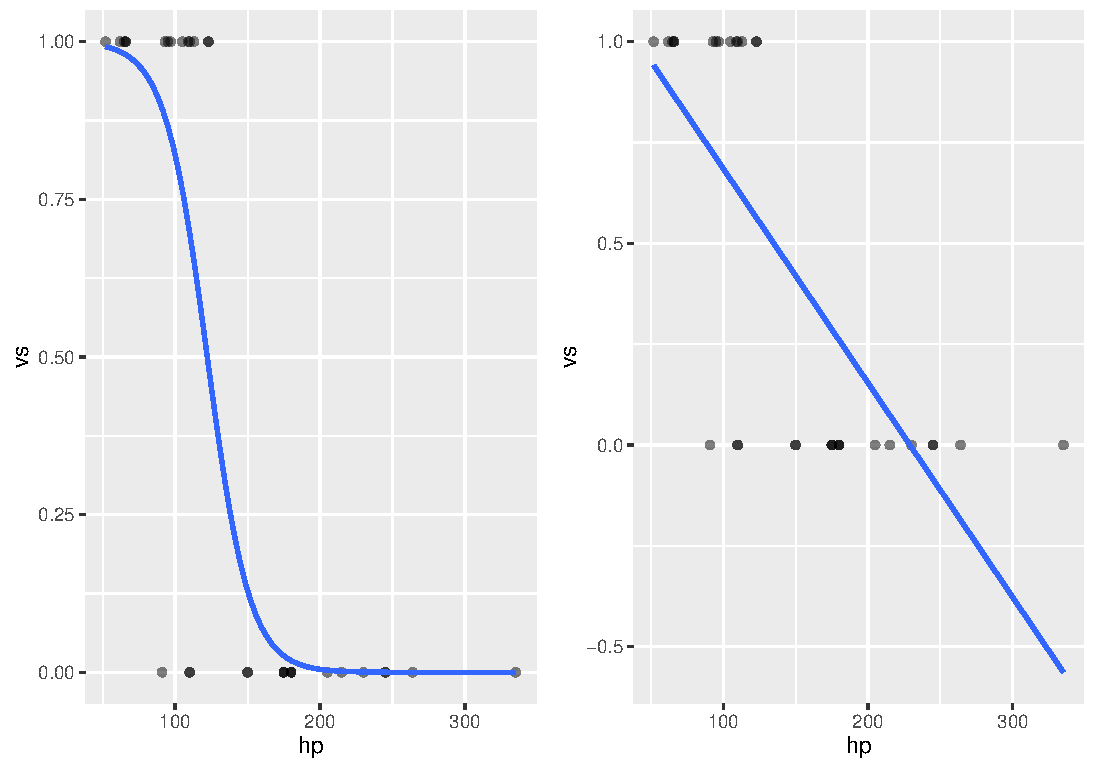
\includegraphics[width=0.75\textwidth]{figures/linear-vs-logistic-example.pdf}
    \caption[Linear versus binomial regression for a binary response.]{Illustrative example of fitting a linear model (to the right) versus a generalized (binomial) linear model (to the left) when the response is binary. The data used is from the standard \texttt{mtcars} set provided by R \autocite{r-core-team}. The response is the engine type (\texttt{vs}), either V-shaped or straight, and the covariate is gross horsepower (\texttt{hp}).}
    \label{fig:illustrative linear-binomial difference}
\end{figure}

Binomial regression is a generalized linear model (GLM). In GLMs, we assume that the response follows a distribution of the exponential family, such as the binomial, Poisson, exponential, or beta distribution. The expected value of the response links to a linear predictor $\bm\eta$ through a link function. More precisely, a GLM can be written as
\begin{equation}
g(\operatorname{E}[\bm Y | \bm X]) = g(\bm \mu) = \bm \eta = \bm X \bm \beta \ ,
\label{eq:glm definition}    
\end{equation}
where $g$ is the link function, $\bm\eta$ is the linear predictor, $\bm\mu$ is the expected value of the distribution of $\bm Y | \bm X$, and $\bm X$ and $\bm\beta$ are as previously defined. For the example of binary binomial regression, we get $\bm Y | \bm X \sim \operatorname{Bern}(\bm\mu)$, that is, $\bm Y | \bm X$ is assumed to have a Bernoulli distribution with mean $\bm\mu$. The common link functions for binomial regression are the logit, probit, and cloglog (complementary log-log) links, and are provided in \autoref{tab:link functions}.

Extending on the idea of an LMM, we have generalized linear mixed models (GLMMs) whose linear predictor $\bm\eta$ can include random effects, in addition to fixed effects. In general, a GLMM will have the form
\begin{align}
    \bm \eta &= \bm X\bm\beta + \bm U \bm \gamma \ , \nonumber \\
    \bm \mu &= g^{-1}(\bm\eta) \ ,  \\
    \bm Y | \bm X &\sim \mathcal D(\bm\mu, \bm\theta) \ , \nonumber
    \label{eq:general glmm}
\end{align}
for a distribution $\mathcal D$ of the exponential family with expected value $\bm\mu$ and (potentially additional) parameters $\bm\theta$.

\begin{table}
    \centering
    \begin{tabular}{ll}
    Link function     & Expression  \\ \midrule
    Logit   & $\log(y_i/(1-\log(y_i)))$ \\
    Probit  & $\Phi^{-1}(y_i)$ \\
    Cloglog & $\log(-\log(1-y_i))$
    \end{tabular}
    \caption[Link functions for binomial regression]{Most common link functions for binomial regression. Here, $\Phi$ is the cumulative density function of a standard normal distribution, $\mathcal N(0,1)$.}
    \label{tab:link functions}
\end{table}

\section{Models in quantitative genetics} 
\label{sec:theory:qg models}
We will use the animal model, which is a specific GLMM, to estimate the additive genetic variance. For context, we first introduce the infinitesimal and threshold model.

\subsection{The threshold model}
\label{sec:theory:threshold model}
The infinitesimal model in quantitative genetics assumes that any phenotypic trait is influenced by an infinite number of loci, all of which have some infinitesimal effect. In simpler terms, the trait of an offspring is Gaussian around the mean of its two parents with a variance independent of the values of the parents \autocite{barton2017}. The motivation behind this modeling choice dates back to \textcite{galton1886}, suggesting a law of ancestral heredity, where the phenotype is decided as the sum of geometrically declining contributions from parents and further up the pedigree. Each ancestor had a probability $p$ of passing the trait to the next generation. This idea is equivalent to the framework we use today, which is an additive genetic trait with the heritability concept replacing, and generalizing, the probability $p$ \autocite{bulmer1998}.

The infinitesimal model motivates us to use a normal distribution with a random effect. However, Gaussian models struggle to provide accurate predictions of binary phenotypes. To remedy this, the infinitesimal model can be extended to allow for more complex trait modeling, namely through the threshold model. Rather than trying to model a specific trait, we consider a latent trait, also called the liability, with a normal distribution. In the example of modeling a binary trait, for a given threshold $M$, the values attained below $M$ are cast to the one binary category, and all values above are set to the latter. \autoref{fig:theory:illustration-threshold} shows an illustration of the threshold model.
\begin{figure}
    \centering
    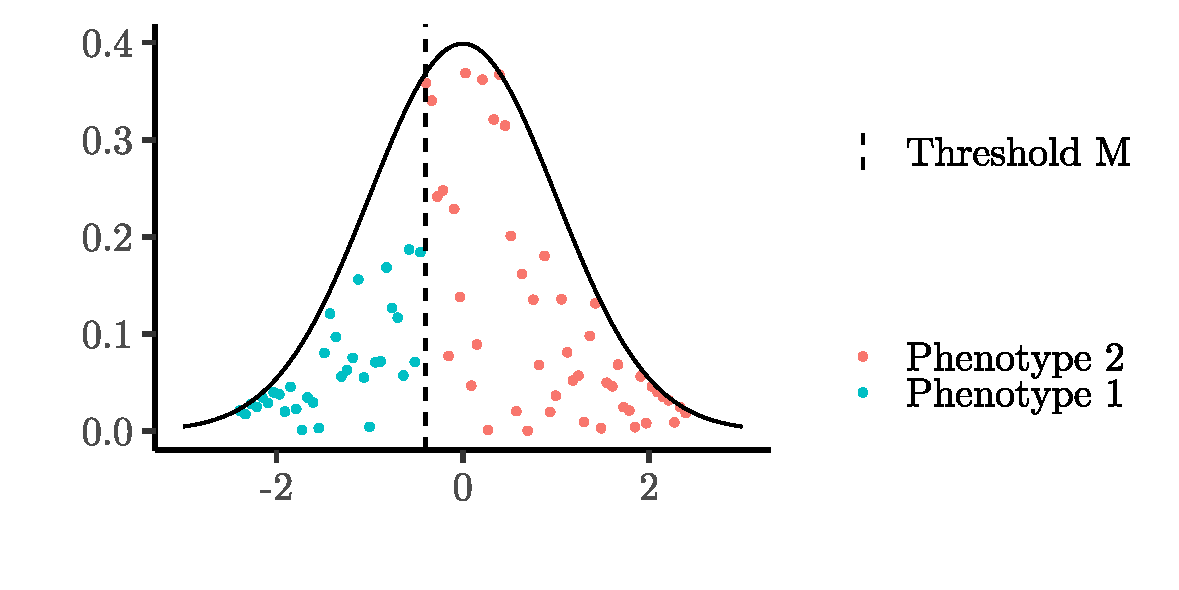
\includegraphics[width=0.75\textwidth]{figures/illustration_thresholdmodel.pdf}
    \caption[Illustration of the threshold model]{Illustration of the threshold model for a binary phenotypic trait. The blue points are realizations of the normal distribution less than the threshold value $M$ and thus belong to phenotype 1. Consequentially, the realizations above $M$ are the red points and belong to phenotype 2.}
    \label{fig:theory:illustration-threshold}
\end{figure}
The heritability computed from the liability trait can be transformed into an observation-scale heritability using the relation
\begin{equation}
h^2_{\text{liab}} = \frac{p(1-p)}{t^2}\;h^2_{\text{obs}} \ ,
\label{eq:heritability for threshold model}
\end{equation}
where $p$ is the proportion of one of the binary phenotypes in the population, and $t$ is density in $\mathcal N(0,1)$ at the $p$th quantile \autocite{dempster1950heritability, de2018quantitative}. The idea of the threshold model has been extended further into a multiple threshold model; see, for instance, \textcite{reich1972use}.

An important result is that \eqref{eq:heritability for threshold model} can be used for Gaussian models fitted to a binary trait when the binary trait is relatively well balanced \autocite{vanvleck1972, elston1977}. This result suggests that a linear (mixed) model can be sufficient to model binary traits if one scales the outcome by a scalar value dependent on the data. Note that \textcite{elston1977} mention that the variation in liability among groups (in terms of the response) should be small for the approximation to be valid. There is also little to no literature exploring the stability of the approximation when including fixed effects in the model.

\subsection{The animal model} \label{sec:theory:animal model}

The animal model is a mixed model that incorporates genetic information as a variance-covariance structure in a random effect. The model can use information from a complex pedigree encoded in a matrix, to estimate the causal components of the phenotypic variance \autocite{kruuk2004}. Whereas alternatives often must assume that there is no assortative mating, inbreeding, or selection, the animal model can account for all three. In a Gaussian case, the animal model can be expressed as the linear mixed model
\begin{align}
    \label{eq:animal model gaussian}
        \bm Y &= \bm X\bm\beta + \bm Z_a \bm a + \bm Z \bm u + \bm \varepsilon \ , \\
        \bm a &\sim \mathcal N(\bm 0,\bm A \sigma^2_A) \ , \nonumber \\
        \bm \varepsilon & \sim \mathcal N(\bm 0,\bm I \sigma^2_E) \ , \nonumber
\end{align}
where $\bm Y$ is the phenotypic trait of interest, $\bm a$ are called the breeding values, or the (total) additive genetic merit, and $\bm \varepsilon$ are the errors. Furthermore, $\bm X\bm \beta$ are the intercept and fixed effects, and each $\bm Z_j u_{ji}$ are the random effects other than the breeding values.

% \subsubsection{Additive genetic relationship matrix}
A key component of the animal model is the additive genetic relationship matrix $\bm A$.
Before defining $\bm A$, we define the coefficient of ancestry, $\Theta_{ij}$, to be the probability that an allele drawn from individual $i$ is the same as an allele from individual $j$. Then we have that $\Theta_{ii}$, that is, self-relatedness, is $\frac12$ and if $i$ and $j$ have a parent-offspring relationship, $\Theta_{ij}=\frac14$. We can then define $\bm A$ so that each $A_{ij} = 2\Theta_{ij}$.
In terms of notation, the total phenotypic variance on the observed scale will be written as $\sigma^2_P$, which is the sum of additive genetic variance, environmental and / or residual variance. Recall that heritability is the proportion of phenotypic variance explained by the additive genetic variance, which now can be expressed mathematically as
\begin{equation}
 h^2_\text{obs} = \frac{\sigma^2_A}{\sigma^2_P} \ .
\end{equation}


\subsection{The animal model for non-Gaussian traits}
\label{sec:theory:interpret heritability}
The threshold model has been used for binary and, in general, categorical traits.
One can show that there is an equivalence between a binomial GLMM whose link function is the probit link, and the threshold model \autocite{de2016general}.
With the extensions to GLMMs, we also have a broader framework that can accurately model non-Gaussian traits.

Specifically, we use a GLMM such as a binomial model with a probit link for the case of a binary trait. Although a probit-based animal model has a better predictive power than a Gaussian animal model, the nonlinearity of the link functions confounds the actual biological values of interest. To illustrate the scales more clearly, we consider a simple binomial probit animal model by
\begin{align}
\label{eq:theory:binom AM latent}
    \bm \eta = \beta_0 + \bm a \ ,  \\
    \bm a \sim \mathcal N(\bm 0, \bm A \sigma^2_A) \ ,\\
    \bm \mu = \Phi(\bm \eta) \ ,\\
    \bm Y | \bm X \sim \operatorname{Bern}(\bm \mu) \ . 
\end{align}
The estimated variance components $\hat\sigma^2_A$ in the model are on the same scale as \eqref{eq:theory:binom AM latent}, namely the latent scale, meaning that the variance is additive on the linear predictor's scale. However, it is no longer additive in relation to observed values, which follow a Bernoulli distribution whose mean is linked through the nonlinear function $\Phi$, that is, the cumulative density function for $\mathcal N(0,1)$. We also illustrate this concept in \autoref{fig:theory:illustration-probit-fitted-values}, where the posterior latent fitted values are shown with the true observations. While the fitted values on the latent scale are far from the true observations, passing the inverse of the link function will obtain the \textit{expected} scale, which reflects the phenotypic mean. However, as apparent in the same figure, none of these scales is the same as the observed data, which are binary realizations of a Bernoulli distribution. In summary, since the link function $g$ is nonlinear, we get a non-additive genetic variance.

\begin{figure}
    \centering
    \begin{subfigure}{0.8\textwidth}
    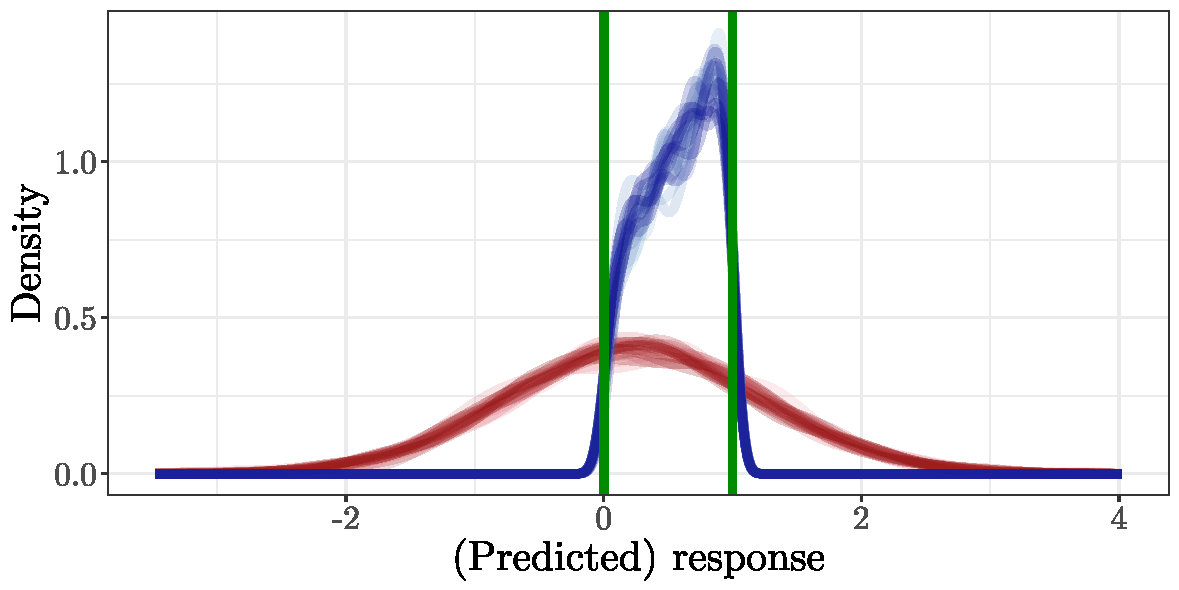
\includegraphics[width=\textwidth]{figures/illustration_probit_scales_fitted_values.pdf}
    \end{subfigure}
    \begin{subfigure}[b]{0.4\textwidth}
        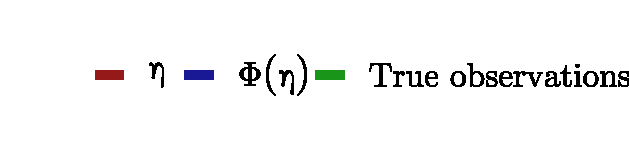
\includegraphics[width=\textwidth]{figures/illustration_probit_scales_fitted_values_legend.pdf}
    \end{subfigure}
    \caption[Illustration of fitted values for a probit animal model]{Illustrative figure showing the fitted values obtained in a binomial probit model. The red lines, $\eta\in(-\infty, \infty)$, are the marginal fitted values, i.e., the fitted values on the latent scale. By using the inverse of the link function, we obtain the dark blue estimate $\Phi(\eta)\in(0,1)$, which can be interpreted as the expected scale. Lastly, the green lines show the true observations $y\in\{0,1\}$. The estimates ($\eta$ and $\Phi(\eta)$) show $20$ posterior samples of these estimates, hence their blurry shape compared to the true observations.} \label{fig:theory:illustration-probit-fitted-values}
\end{figure}

We have motivated the interest in applying animal models %in wild populations
to get heritability estimates. However, only reporting the heritability on the latent scale is not viable, as inferring parameters on the observation scale should be the standard approach \autocite{de2018quantitative}. This raises the issue of how one can get usable estimates on the original observation scale when using nonlinear models.
There are several potential remedies to obtain an estimate comparable to the observation scale, one of them by introducing \textit{ link variance}. By sending the linear predictor through the nonlinear inverse link function $g^{-1}(\eta_i)$, one introduces variance. Traditionally, this is captured by adding a term to the denominator in the heritability estimate, for instance in the probit case
\begin{equation}
    h^2_{\Phi} = \frac{\sigma^2_A}{\sum_i \sigma^2_i +1} \ ,
    \label{eq:link variance h2 phi}
\end{equation}
where $\sum_i \sigma^2_i$ is the sum of the variance components from the random effects. Including the term $1$ in the denominator captures the link variance for a probit model and attains the same scale as would be achieved using the threshold model, that is, the \textit{liability scale}. Similarly, the link variance in a binomial model with a logit link is $\pi^2/3$ and the cloglog link is $\pi^2/6$ \autocite{nakagawa2017}. Although this method is easy to use, it does not address the issue of fixed effects influencing heritability and does not yield heritability estimates on an observation scale.

In wild populations, we must interpret heritability as conditioned on any fixed effects chosen in the model \autocite{wilson2008}. To remedy this, \textcite{de2016general} introduces a method that attempts to obtain heritability estimates on the observation scale by averaging over fixed effects. The algorithm is based on the same three hierarchical scales introduced by \autoref{fig:theory:illustration-probit-fitted-values}, namely, the latent scale, the expected scale and the observation scale.
%The latent scale is the direct output of the model, for instance, the $\bm\hat\beta$ or the variance components $\hat\sigma^2_A$ and $\hat\sigma^2_E$. The expected scale is simply the inverse link function applied to the parameters on the latent scale. Thus, the observation scale consists of realizations from the assumed distribution given the expected values defined from the expected scale and potentially other parameters (such as variance).
The primary goal will be to convert from the latent scale to the observation scale, as presented below. 

\subsubsection*{A general back-transformation algorithm}
\textcite{de2016general} also suggests general formulae, both tackling the back-transformation of variables onto the observation scale and providing a method to average over the fixed effects. The purpose of averaging over fixed effects is to attempt to remove the heritability's dependence on model choices of fixed effects. 

The algorithm is detailed in \autoref{alg:qgglmm}. In the algorithm, $g^{-1}$ is the inverse link function for a given model, $\sigma^2_{RE}$ is the sum of variance from all random effects, $f_{\mathcal{N}}(x;\mu,\sigma^2)$ is the density function for the distribution $\mathcal{N}(\mu,\sigma^2)$, and $\mathcal{V}$ is a distribution-specific variance function. 


\begin{algorithm}
\caption{General method for observation-scale heritability $h^2_\Psi$.} \label{alg:qgglmm}
    \begin{algorithmic}
    \State \textbf{Input:} Latent additive genetic variance $\sigma^2_{A,l}$ and total phenotypic variance $\sigma^2_{RE,l}$, either intercept $\mu$ or \texttt{predict} (latent marginal estimates). Optional: $w$, width for integration.
    \If{\texttt{predict} given but not $\mu$}
        \State $\Tilde{\bm\mu} \gets$ \texttt{predict}
    \Else
        \State $\Tilde{\bm\mu} \gets [\mu, \dots, \mu]^\top$ \algorithmiccomment{Such that $\Tilde{\bm\mu} = [\Tilde{\mu}^{(1)}, \dots, \Tilde{\mu}^{(N)}]^\top$}
    \EndIf
    \State $\bar z \gets \frac1N\sum_{i=1}^N \int_{\tilde\mu^{(i)} - w \sqrt{\sigma^2_{RE,l}}}^{\tilde\mu^{(i)} + w \sqrt{\sigma^2_{RE,l}}} g^{-1}(x)f_{\mathcal N}(x; \mu=\tilde\mu^{(i)},\sigma^2=\sigma^2_{RE,l})dx$
    \State $\sigma^2_{RE, exp} \gets \left(\frac1N\sum_{i=1}^N \int_{\tilde\mu^{(i)} - w \sqrt{\sigma^2_{RE,l}}}^{\tilde\mu^{(i)} + w \sqrt{\sigma^2_{RE,l}}} \left(g^{-1}(x)\right)^2 f_{\mathcal N}(x; \mu=\tilde\mu^{(i)},\sigma^2=\sigma^2_{RE,l})dx\right)-\bar z^2$
    \State $\sigma^2_{RE, dist} \gets \frac1N\sum_{i=1}^N \int_{\tilde\mu^{(i)} - w \sqrt{\sigma^2_{RE,l}}}^{\tilde\mu^{(i)} + w \sqrt{\sigma^2_{RE,l}}} \mathcal{V}(x) f_{\mathcal N}(x; \mu=\tilde\mu^{(i)},\sigma^2=\sigma^2_{RE,l})dx$
    \State $\sigma^2_{RE,obs} \gets \sigma^2_{RE, exp} + \sigma^2_{RE, dist}$
    \State $\Psi \gets \frac1N\sum_{i=1}^N \int_{\tilde\mu^{(i)} - w \sqrt{\sigma^2_{RE,l}}}^{\tilde\mu^{(i)} + w \sqrt{\sigma^2_{RE,l}}} \frac{\partial g^{-1}(x)}{\partial x} f_{\mathcal N}(x; \mu=\tilde\mu^{(i)},\sigma^2=\sigma^2_{RE,l})dx$
    \State $h^2_{\Psi} \gets \frac{\Psi^2 \sigma^2_{A,l}}{\sigma^2_{RE,obs}}$
    \State \textbf{Returns: } $h^2_{\Psi}$
    \end{algorithmic}
\end{algorithm}

In the case where we have a binomial probit model, the sequence obtains a closed-form solution, given by \autoref{alg:qgglmm-probit}, and will be significantly faster than, for instance, a binomial logit model.

\begin{algorithm}
\caption{Observation-scale heritability for a binomial probit model.} \label{alg:qgglmm-probit}
    \begin{algorithmic}
    \State \textbf{Input:} Latent additive genetic variance $\sigma^2_{A,l}$ and total phenotypic variance $\sigma^2_{RE,l}$, either intercept $\mu$ or \texttt{predict} (latent marginal estimates).
    \If{\texttt{predict} given but not $\mu$}
        \State $\Tilde{\bm\mu} \gets$ \texttt{predict}
    \Else
        \State $\Tilde{\bm\mu} \gets [\mu, \dots, \mu]^\top$ \algorithmiccomment{Such that $\Tilde{\bm\mu} = [\Tilde{\mu}^{(1)}, \dots, \Tilde{\mu}^{(N)}]^\top$}
    \EndIf
    \State $p \gets \frac{1}{N} \sum_{i=1}^N 1-\Phi(0;\mu=\tilde\mu^{(i)},\sigma^2=\sigma^2_{RE,l}+1)$
    \State $\sigma^2_{RE,obs} \gets p(1-p)$
    \State $\Psi \gets \frac{1}{N}\sum_{i=1}^N f_{\mathcal N}(0;\mu=\tilde\mu^{(i)},\sigma^2=\sigma^2_{RE,l}+1)$
    \State $h^2_{\Psi} \gets \frac{\Psi^2 \sigma^2_{A,l}}{\sigma^2_{RE,obs}}$
    \State \textbf{Returns: } $h^2_{\Psi}$
    \end{algorithmic}
\end{algorithm}

\section{Bayesian inference and INLA}

\subsection{The Bayesian statistical modeling framework}

We can consider two main frameworks for statistical modeling: a frequentist approach and a Bayesian approach. When modeling with a frequentist approach, we assume that the parameters in a model have one true value, whereas, in a Bayesian approach, we interpret them as stochastic with their own distributions. The prior distribution in the Bayesian framework represents the knowledge that we have in the model before we observe the data itself. Using an appropriate prior can improve the accuracy of the model. Another key component in Bayesian statistics is that the methods used provide a probabilistic interpretation of the fitted values, which is helpful for further inference in the model of interest. In terms of notation, we define the operator $\operatorname{MAP}[\bm X]$ as the maximum a posteriori of a random variable $\bm X$ with a posterior distribution and represents the mode of the posterior distribution computed for $\bm X$.
Simulation studies have also shown that in the case of the estimation of heritability of binary traits, the use of Bayesian models is the most effective \autocite{devillemereuil2013}, further motivating the use of Bayesian frameworks.

\subsubsection*{Penalized complexity priors}

A suitable choice of priors can significantly improve the performance of a model, while choosing unsuitable priors can increase the bias in the model. Thus, choosing prior distributions in a Bayesian model is not a trivial task. When there is little prior knowledge, noninformative priors, and improper priors (such as the uniform distribution) can be used. An improper prior is any prior distribution that integrates to a non-finite value. However, improper priors can also lead to other issues, such as improper posterior distributions. 

For this thesis, we will be using penalized complexity (PC) priors \autocite{simpson-pcpriors}. By introducing penalized complexity priors, simpler and more interpretable models will be prioritized, while more complex models that tend to overfit the data will be penalized. PC priors require only two parameters, namely $U$ and $\alpha$ where $0<\alpha<1$. Informally, the prior $\operatorname{PC}(U, \alpha)$ on some parameter $\bm\theta$ is expressed so that the probability $\operatorname{Pr}(\bm\theta \le U) = 1-\alpha$.

For the case of a random effect $[a_1, \dots, a_n]^\top = \bm a \sim \mathcal N(\bm 0, \bm A \sigma^2_A) = \mathcal{N}(\bm 0,\bm A \tau_A^{-1})$, the PC prior becomes a type-2 Gumbel distribution with respect to $\lambda$,
\begin{equation}
    \pi(\tau_A) = \frac{\lambda}{2} \tau^{-3/2} \exp(-\lambda\tau_A^{-1/2}),\quad \tau_A>0,\; \lambda>0 \ ,
\end{equation}
and with $\operatorname{Pr}(\tau_A^{-1/2} \le U)=1-\alpha$, we obtain $\lambda=-\ln(\alpha)/U$ \autocite{simpson-pcpriors}. PC priors have a parameterization so that $U$ resembles the standard deviation, for example, a PC prior $\operatorname{PC}(1,0.05)$ for the breeding values $\bm a$ would resemble $\operatorname{Pr}(\sigma_A \le 1) = 0.95$.

\subsection{The INLA computing scheme}
INLA is an abbreviation for the term integrated nested Laplace approximation and is an alternative to fitting Bayesian models using Markov chain Monte Carlo (MCMC). INLA is a faster alternative to obtain posterior distributions for latent Gaussian models. In this brief review of INLA, we use the notation and definitions provided in \textcite{inla-lecturenotes}.

A latent Gaussian model is a relatively broad class of models consisting of observations $\bm y$, a latent field $\bm x$, and hyperparameters $\bm \theta$ with a partition $\bm\theta = (\bm \theta_1, \bm \theta_2)^\top$. We have that

\begin{align}
    \bm y | \bm x \sim \prod_i \pi(y_i | x_i, \dots, \bm \theta_1) \label{eq:inla:lgm1} \\
    \bm x | \bm \theta_1 \sim \mathcal N(0, \bm Q(\bm\theta_2)^{-1}), \label{eq:inla:lgm2} \ ,
\end{align}
where \eqref{eq:inla:lgm1} implies that $\bm y$ is conditionally independent given $\bm x$ and $\bm \theta_1$ and $\pi(\cdot)$ indicates the distribution of a random variable, and $\bm Q$ in \eqref{eq:inla:lgm2} is the precision matrix for the latent field $\bm x$. Furthermore, we assume that $\bm x$ is a Gaussian Markov Random Field (GMRF). To obtain effective computations within the INLA framework, the precision matrix $\bm Q$ should be sparse. Within the context of the animal model, $\bm Q = \bm A^{-1}$, which has been shown to be sparse \autocite{steinsland2010utilizing}. The linear predictor in a latent Gaussian model is

\begin{equation}
    \eta_i = \alpha + \sum_{l} f_i(u_{l,i}) + \sum_k \beta_k z_{k,i} + \varepsilon_i \ ,
\end{equation}
which we can use to express both linear models, GLMs, GLMMs, and more complex models like geostatistical models. 

\subsubsection*{The INLA computing scheme} 

The first step of the INLA computing scheme is to obtain estimates for the marginal hyperparameter distribution. That is, $\pi(\bm\theta_j | \bm y) = \int \pi(\bm \theta | \bm y) d\bm\theta_{-j}$, which we compute numerically. The notation $\bm\theta_{-j}$ means all elements of $\bm\theta$ except $j$. In particular, we can approximate the marginal hyperparameter distribution using the expanded form \autocite{gentleINLA}
\begin{equation}
    \pi(\bm\theta|\bm y) \approx \left.\frac{\pi(\bm y | \bm x, \bm \theta) \times \pi(\bm x | \bm \theta) \times \pi(\bm \theta)}{\Tilde{\pi}_G(\bm x | \bm \theta, \bm y)}\right|_{\bm x = \operatorname{MAP}[\pi(\bm x |\bm \theta, \bm y)]} \ ,
\end{equation}
where $\Tilde{\pi}_G$ is the GMRF approximation.
With these, INLA selects suitable support points (for non-scalar $\bm\theta$) with Newton-like numerical methods such that each $\bm\theta_k$ has weight $\Delta_k$ \autocite{gentleINLA}.

With the marginal hyperpriors, we can get the distribution of the latent space by $\pi(x_i | \bm y)=\int \pi(x_i|\bm\theta,\bm y)\times\pi(\bm\theta|\bm y)d\bm\theta$ with additional Laplace approximations, given that they are not Gaussian. The Laplace approximation can be done using either a full Laplace approximation or a simplified version based on a skew-normal distribution to a series expansion of $\Tilde{\pi}(x_i|\bm\theta, \bm y)$ \autocite{inla-lecturenotes}.
Lastly, we can obtain the posterior estimate $\tilde{\pi}(x_i | \bm y)$ as
\begin{equation}
    \Tilde{\pi}(x_i | \bm y) = \sum_k
    \Tilde{\pi}(x_i | \bm \theta_k, \bm y) \times \tilde{\pi}(\bm\theta_k|\bm y) \times \Delta_k \ .
\end{equation}
The package R-INLA \autocite{inla2009} implements the computing scheme and will be used to fit all models in this thesis.


% \section{Notation}
% Placeholder in case I need to define new notation...
